\documentclass[10pt,conference,compsocconf]{IEEEtran}
% \topmargin=0.cm
%\addtolength{\textheight}{1.75cm}

\usepackage{caption}
\usepackage{subcaption}
\usepackage{listings}
\usepackage{hyperref}
\usepackage{graphicx}	% For figure environment
\usepackage{tabularx}
\usepackage{booktabs}	% http://ctan.org/pkg/booktabs
\usepackage{amssymb}	% For math symbols
%\usepackage[labelformat=empty]{caption}
\usepackage{float}
\newcommand{\tabitem}{~~\llap{\textbullet}~~}
\usepackage[margin=0.5in]{geometry}

\begin{document}
\title{%2\textsuperscript{nd} Project Report: 
Twitter Sentiment Classification}

\author{ \textbf{\texttt{[Memory Error]}}
	Concetto Emanuele Bugliarello, Manik Garg and Zander Harteveld \\
  \textit{Pattern Classification and Machine Learning (CS-433), Second Project, Fall Semester 2016, EPFL, Switzerland}\\
  \texttt{\{emanuele.bugliarello, garg.manik, zander.harteveld\}@epfl.ch}
}

\maketitle

\begin{abstract}
%TODO - full summary of the report
Social media platforms such as Twitter are a rich source of text examples expressing positive and negative sentiment. 
In this paper, we investigate the classification accuracy achieved by different learning algorithms in determining sentiments associated to tweets.
Through data pre-processing and hyperparameter tuning, we report our computationally light TF-IDF Logistic Regression model, scoring 87.00 $\%$ accuracy in the EPFL ML Text classification challenge on Kaggle.
%in top \texttt{10}
.
\end{abstract}
\vspace{0cm}
\section{Introduction}
Sentiment analysis is an interesting problem aiming to give a machine the ability to understand the emotions and opinions expressed by humans. This is an extremely challenging task due to the complexity of human language, which makes use of rhetorical devices such as sarcasm or irony.\\
Twitter is a popular ``micro-blogging" social networking website for conveying opinions and thoughts, and thus a successful sentiment classification model based on Twitter data could provide interesting trends regarding prominent topics in the news or popular culture. For example, one could gauge the popular opinion of a politician by calculating the sentiment of all tweets containing the politician's name. Sentiment analysis in Twitter is a significantly different paradigm than past attempts at sentiment analysis through machine learning since its users are only allowed to post short status updates of less than 140 characters (``tweets"). Moreover, as in most online social networks, users create their own words and spelling shortcuts, that, in addition to misspellings, slang, and abbreviations, make this task even more challenging.\\
The aim of this project is to build an accurate sentiment analyzer for tweets. 
That is, given a user-generated status update, our classification model determines whether the given tweet reflects a positive or negative opinion on the user’s behalf.\\
In this report, we will discuss about the methods for building such sentiment analyzer including data pre-processing, creation of word vector representations and hyperparameter optimization for different classifiers.

\vspace{0cm}
\section{Data}
The dataset we use to train and test our classifiers is the one provided for the EPFL Machine Learning text classification challenge on Kaggle\cite{KaggleEPFL}.
The dataset consists of two small sets of training tweets for each of the two classes\footnote{Positive/negative sentiment associated to the tweet.} (100,000 tweets each), two complete sets of training tweets for each of the two classes (1.25M tweets per class) and a test set (10,000 tweets).
%\subsection{Kaggle Set}
%We were given two sets of 1'250'000 tweets, one containing negative evaluated tweets (contained a negative smiley) and the other positive tweets (contained a positive smiley), making a total of 2'500'000 tweets for training. As this is a huge amount of data and thus computationally expensive, we first explored and tried different methods with a smaller set of 200'000 tweets, half of them evaluated positive and half of them negative.
%\subsection{Enlarged Set}
%We ran the cv on truncated set and saw that the predictions were better on full dataset. As one can easily find more pre-labeled tweets, we were able to enlarge our training set. (This is as more training data will very likely increase the classification accuracy)--> \textbf{true only when our dataset suffers from high variance... which may be the case so we need to put a plot or we can say it learns more words??}\\

The Twitter Sentiment Analysis Dataset obtained from \textit{http://thinknook.com/twitter-sentiment-analysis-training-corpus-dataset-2012-09-22/} contains 1,578,627 classified tweets based on data from the following two sources:\\
University of Michigan Sentiment Analysis competition on Kaggle\\
Twitter Sentiment Corpus by Niek Sanders\\	

Each row is marked as \texttt{1} for positive sentiment and \texttt{0} for negative sentiment that we changed to \texttt{-1} to maintain consistency with our labels \texttt{$\{$1,-1$\}$}.
% \vspace{0.3cm}


\iffalse
%\begin{frame}{}
 %   \begin{figure}[h!]
  %      \begin{minipage}[t]{\linewidth}
   %         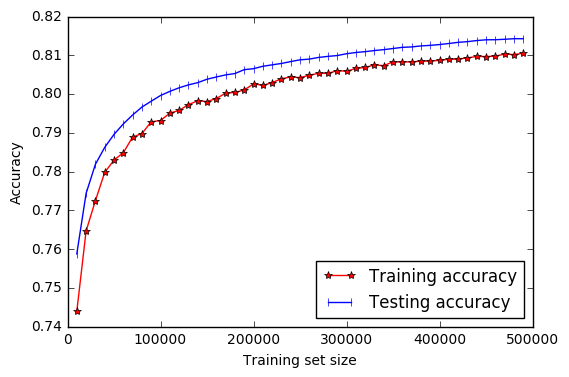
\includegraphics[width=\textwidth]{plots/data_set_size_vs_accuracy.png}
  %          \caption{\small \textbf{a}}
  %          \label{fig:a}
  %      \end{minipage}
  %      \begin{minipage}[t]{0.32\linewidth}
  %          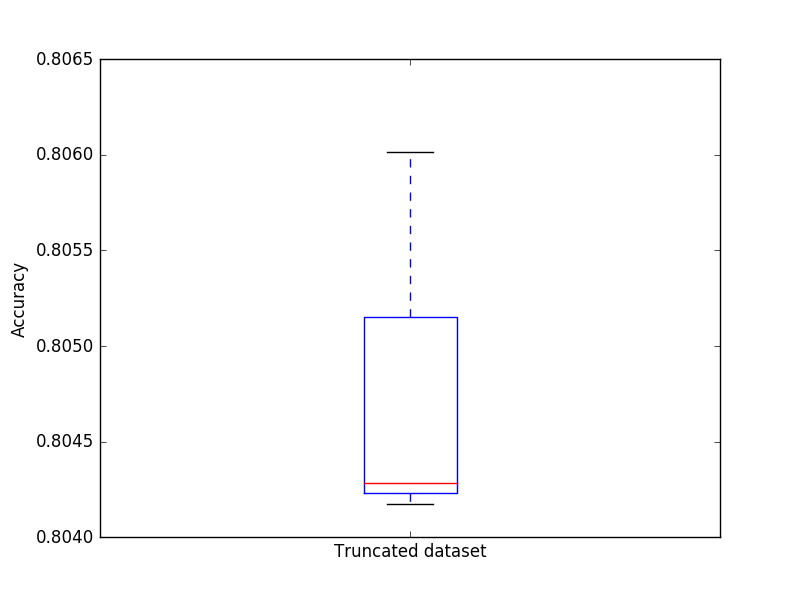
\includegraphics[width=\textwidth]{plots/trunc.png}
  %          \caption{\small \textbf{b}}
  %          \label{fig:b}
  %      \end{minipage}
  %    \begin{minipage}[t]{0.32\linewidth}
  %          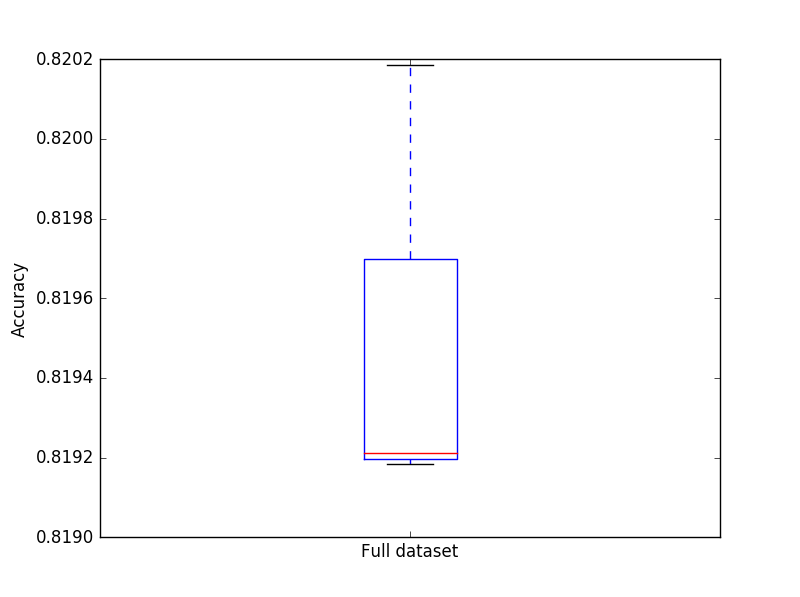
\includegraphics[width=\textwidth]{plots/full.png}
  %          \caption{\small \textbf{c}}
  %         \label{fig:b}
       \end{minipage}
        \begin{minipage}[t]{0.32\linewidth}
            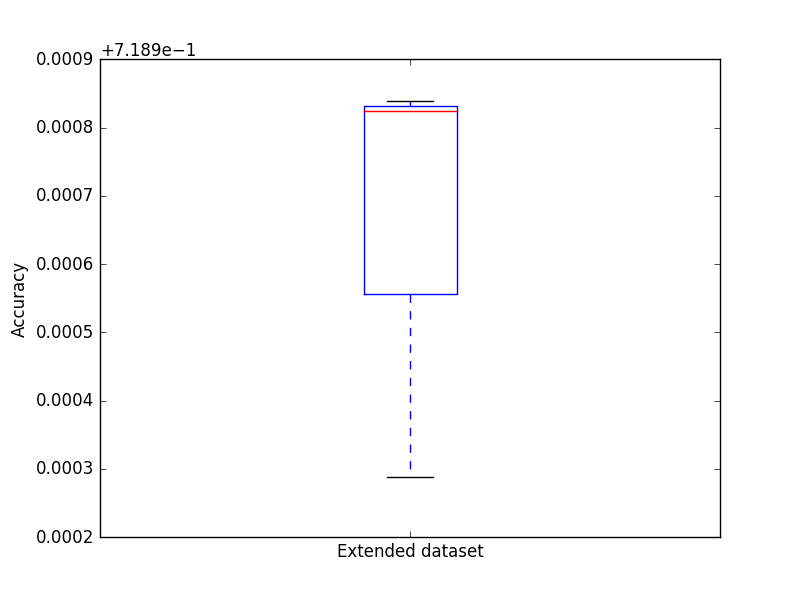
\includegraphics[width=\textwidth]{plots/extended.png}
            \caption{\small \textbf{d}}
            \label{fig:b}
        \end{minipage}
        \hspace{0.5cm}
        \vspace{0.3cm}
        \caption{\textbf{Figure 1:} (a) Variation of dataset size on accuracy achieved on validation set from default TF-IDF logistic (b) boxplot of 3-fold CV for given truncated dataset; (c) boxplot of 3-fold CV for given full dataset; (d) boxplot of 3-fold CV for extended dataset}
    \end{figure}
\end{frame}
\fi

\section{Methodology}
In the following sections, we analyze different classifiers: Logistic Regression (LogReg), multinomial Naive Bayes (MNB) and Support Vector Machine (SVM) with the linear kernel. 
To evaluate the performances of these classifiers, we run experiments on the provided small sets of labeled tweets, splitting them in train (80\%) and test (20\%) sets. 
The learning is then performed using a 3-fold cross validation (CV), such that, in each fold, 2 partitions are used for training and 1 partition for validation. 
Testing is then done on the completely held-out set. 
Standard deviations (std) of the training set are reported from validation accuracies around 3-fold CV. 
On the other hand, std on testing set are reported from the accuracy on test set and mean validation accuracy from the 3-fold CV. 
The only metric used to assess the performances of the classifiers, in accordance with the competition's objective, is their accuracy in predicting correct labels. 
\subsection{Feature generation}
To build an accurate text classifier, it is crucial to find a good feature representation of the input text. Out of the numerous text feature engineering methods, we discuss two of them in this following section. 
%As the traditional ``bag-of-words model'' does not catch the meaning of a tweet, we focus on a more advanced methodology: TF-IDF \textbf{does TF-IDF catch the meaning of tweets?}.\\
%\iffalse
%\subsubsection{GloVe (Stanford University)}
\begin{itemize}
\item \textbf{GloVe (Stanford University).}
%The Global Vectors for Word Representation (GloVe)~\cite{pennington2014glove} is an unsupervised learning algorithm to generate numerical vectors of words. 
The basic idea behind Global Vectors for Word Representation (GloVe)~\cite{pennington2014glove} is that ratios of word-word co-occurrence probabilities can encode some form of meaning. 
Thus, one can measure the relatedness of two words by computing the Euclidean distance (or cosine similarity) between two word vectors.
\iffalse
\subsubsection{FastText (Facebook)}
The FastText technique~\cite{bojanowski2016enriching,joulin2016bag} takes into account the internal  structure  of  words. Each word is represented as a bag of character n-grams. A vector is computed for each n-gram and these vectors are averaged to give a sentence representation.
\fi
%\subsubsection{TF-IDF}
\item \textbf{TF-IDF.}
Term Frequency - Inverse Document Frequency (TF-IDF) is a common numerical statistic that is intended to reflect the importance of a word to a document in a corpus.
It consists of two terms.
First, the term frequency (TF) measures how frequent a specific term appears in a document. The second term, inverse document frequency (IDF), is computed as the logarithm of the number of documents in the corpus divided by the number of documents where the specific term appears.
It weights down terms occurring very frequently in the corpus and increases the weight of terms that occur rarely; thus giving a measure of how important a term is.

\iffalse
The second term, inverse document frequency (IDF), is computed as the logarithm of the number of documents in the corpus divided by the number of documents where the specific term appears.
It weights down terms occurring very frequently in the corpus and increases the weight of terms that occur rarely; thus giving a measure of how important a term is.
\fi
\end{itemize}
% To compute the TF-IDF, one can use the \texttt{python scikit-learn} implementation\cite{scikit-learn}, which is also directly standardizing the features.

\subsection{Pre-processing}\label{preproIII}
We now present various pre-processing steps suitable for this text classification task.
The dataset provided for the competition has already been pre-processed by (i) replacing user references with a generic token (@XYZ $\rightarrow$ \texttt{<user>}), (ii) replacing URLs with a generic token (\texttt{<url>}), (iii) lowering the text and (iv) adding whitespace around punctuation.\\
Through our error analysis and intuition, we notice several tweet characteristics that could potentially be useful as pre-processing for a TF-IDF feature representation.
The following shows a list of pre-processing steps we have extensively been investigating:
\begin{itemize}
\item \textbf{Remove numbers.} Usually, numbers do not convey any emotions and could thus be stripped away. This is not always true: dates such as 09/11/2001 can clearly identify the polarity of a tweet.
\item \textbf{Stemming}. Stemming is reducing words back to their root word. This might be useful as those words usually have a very similar meaning and can be grouped together.
\item \textbf{Lemmatization.} Lemmatization is determining the lemma of a word based on its intended meaning with the use of a vocabulary and morphological analysis of words. This results in removing inflectional endings only and to return the base or dictionary form of a word.
\item \textbf{N-grams.} N-grams can help detecting the correct meaning of a sentence by including combination of multiple words as tokens. N specifies the number of words in each combination. 
\item \textbf{Remove stop words.} Usually, stop words are extremely common words which would appear to be of little value in helping select documents matching a user need (sentiment classification in our case).
\item \textbf{Remove \texttt{<user>} and \texttt{<url>}.} Any group of words can actually be chosen as the stop words for a given purpose. Thus, due to their high frequency, \texttt{<user>} and \texttt{<url>} can be considered as stopwords and so could be removed from the text.
\item \textbf{Remove the pound sign.} A hashtag may just consist of a single word and thus removing the pound sign (\#) at the beginning of it would improve the TF-IDF weights.
\item \textbf{Group emoticons.} Preserving emoticons and mapping different representations of the same emoticon into one (e.g., \{ :-), : ), ( - :, (: \} $\rightarrow$ \{ :) \}) could let the classifier associate it to a specific polarity.
\item \textbf{Negate verbs.} Inspired by Pang and Lee's sentiment analysis research\cite{not_paper}, stripping out the word ``not'' from tweets and appending the characters “NOT\_” before the following token in a tweet could identify negative feelings associated to otherwise positive words. For instance, ``She does not like me'' would become ``She does NOT\_like me'' and so ``NOT\_like'' would be a new (negative) token.
\item \textbf{Fix common typos.} Typos are very common in tweets and thus fixing the most common ones (e.g., people forget the apostrophe when negating an auxiliary) might correctly identify several instances.
\item \textbf{Replace repeating letters.} By looking at the tweets, it is possible to see that sometimes people repeat letters to stress the emotion (e.g., ``hunggrryyy'', ``huuuuuuungry'' for ``hungry''). Thus, another pre-processing step is to look for two or more repetitive letters in a word and replace them by just two of them.
\end{itemize}
% \vspace{0cm}
\section{Results}
% \noindent \begin{table*}[htbp]
%   \centering
%   \begin{tabular}[c]{|l||l|l|l|}
%   %\begin{tabular}[c]{|l||l|l|l|}
%     \hline
%     Embeddings&Classifier (default sklearn settings)&Accuracy\\
%     \hline
%     &&\\
%     GloVe with $\eta$ = 0.001, $\alpha$ = 0.75, nmax = 100, epochs = 10& & \\
%     \hspace{4mm} \textbullet \space 20 features&Logistic regression&0.5965 $\pm$ 0.00197\\
%     \hspace{4mm} &SVM&0.6083 $\pm$ 0.00140\\
%     \hspace{4mm} \textbullet \space 100 features&Logistic regression&0.6159 $\pm$ 0.00069\\
%     \hspace{4mm} &SVM&0.6041 $\pm$ 0.00165\\
%     TF-IDF& & \\
%     \hspace{4mm} \textbullet \space default&Logistic regression&0.8097 $\pm$ 0.00243\\
%     %\hspace{4mm} &Naive Bayes (Multinomial NB)&0.7651 $\pm$ 0.00042\\
%     \hspace{4mm} &SVM&0.7914 $\pm$ 0.00039\\
%     \hline
%   \end{tabular}
%   \vspace{3mm}
%   \caption{Numerical word representation models on small data set}
%   \label{Baselines_table}
% \end{table*}

\begin{table*}[htpb]
\centering
\resizebox{1.5\columnwidth}{!}{
\tiny\tiny
\begin{tabular}[c]{{l}c*{1}c} 
\hline
\rule{0pt}{2mm}
\textbf{Embeddings}&\textbf{Classifier}&\textbf{Accuracy}\\
\hline
\rule{0pt}{3mm}
GloVe with $\eta$ = 0.001, $\alpha$ = 0.75, nmax = 100, epochs = 10& & \\
\rule{0pt}{2mm}
\hspace{4mm} \textbullet \space 20 features&LogReg&0.5965 $\pm$ 0.00197\\
    \hspace{4mm} &SVM&0.6083 $\pm$ 0.00140\\
\rule{0pt}{2mm}
    \hspace{4mm} \textbullet \space 100 features&LogReg&0.6159 $\pm$ 0.00069\\
    \hspace{4mm} &SVM&0.6041 $\pm$ 0.00165\\
TF-IDF& & \\
\rule{0pt}{1mm}
    \hspace{4mm} \textbullet \space default&LogReg&0.8097 $\pm$ 0.00243\\
    \hspace{4mm} &SVM&0.7914 $\pm$ 0.00039\\
    \hline
\end{tabular}
}
\caption{Numerical word representation models on small data set. Classifiers are from scikit-learn, with default settings.}
\label{Baselines_table}
\end{table*}

In this section we specify the results obtained for each of the methodologies discussed, and the analysis performed in order to construct our final sentiment analysis model.
%\textbf{TODO: THE FOLLOWING ARE NOOOOOT RESULTS!!! PUT THEM BACK TO METHODOLOGY. THOSE ARE NOT METHODOLOGY EITHER...OUR METHODOLOGY IS A GENERALIZED TEXT}
\subsection{Feature generation}
To select the best model for generating numerical word representations, we compare the GloVe word embedding, with both 20 and 100 features per word, with the default instance of TF-IDF from \textit{scikit-learn}\cite{scikit-learn}.
To obtain a first insight into the performances of the models, we perform the training of the obtained word-to-vector matrix and word-frequency-based feature matrix using the LogReg and SVM classifiers from \textit{scikit-learn} without any hyperparameter optimization. 
As it is shown in Table~\ref{Baselines_table}, the best classification results of the raw data are obtained using TF-IDF word vectors. 
We therefore proceed using TF-IDF to optimize data pre-processing and hyperparameter optimization steps for LogReg and SVM classifiers in order to improve their accuracy.
Moreover, the accuracy of a classifier increases with the dataset size, as shown in Fig. \ref{fig:dataset}.\\
% \vspace{0.3cm}
\begin{figure}[h]
%    	\begin{subfigure}[]{0.50\textwidth}
        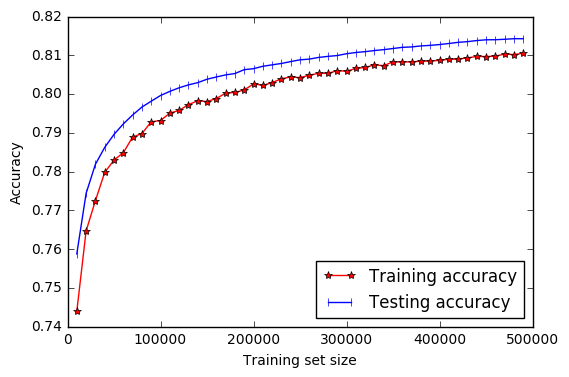
\includegraphics[width=0.965\columnwidth]{plots/data_set_size_vs_accuracy.png}
            \caption{Effect of dataset size on accuracy as observed on test set with default TF-IDF LogReg model.}\label{fig:dataset}
%             \caption{\small}
%             \label{fig:a}
%     \end{subfigure}
    ~ %add desired spacing between images, e. g. ~, \quad, \qquad, \hfill etc. 
      %(or a blank line to force the subfigure onto a new line)
%       \vspace*{-1.5mm}
%     \begin{subfigure}[]{0.50\textwidth}
%         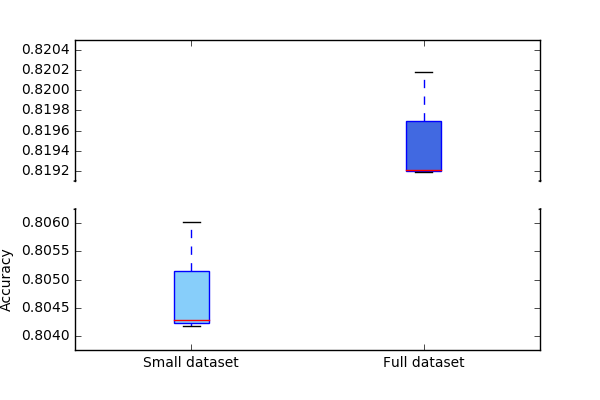
\includegraphics[width=\columnwidth]{plots/nicely_cut_colored.png}
%             \caption{\small}
%             \label{fig:b}
%     \end{subfigure}
    ~ %add desired spacing between images, e. g. ~, \quad, \qquad, \hfill etc. 
    %(or a blank line to force the subfigure onto a new line)
    \
\end{figure}
\vspace{-1cm}
\subsection{Pre-processing}
We now show the additional pre-processing steps, in an aggregating manner, used to obtain the best classification accuracy for each of the aforementioned classifiers.
The baseline pre-processor is referred to the received dataset (having applied the pre-processing steps described in section \ref{preproIII}).
\subsubsection{Dummy}
The baseline classifier is a random classifier that is evaluated on the received dataset without any pre-processing.
As expected, the accuracy of such classifier is around $50\%$. Specifically, $0.5018 \pm 0.0019$ for a 3-fold CV.
\subsubsection{LogReg}
For each additional pre-processing step, a LogReg classifier (with default regularization parameter \texttt{$C$=1}) is trained. 
The pre-processing steps that yielded improvements on test accuracy are listed in Table \ref{tab:logreg_table}. 
Other pre-processing steps yielded lower test set accuracies.
\vspace{-0.19cm}
\begin{table}[H]
\centering
\resizebox{\columnwidth}{!}{
% \tiny
\begin{tabular}{{l}c*{2}c} 
\hline
	            & \textbf{train} & \textbf{test} & \textbf{change} \\
\hline
\rule{0pt}{3mm}
base			& 0.8048$\pm$0.0009	& 0.8097$\pm$0.0024 	& 0.00$\%$	\\
+repeating letters & 0.8227$\pm$0.0015 & 0.8271$\pm$0.0015
    & 1.74$\%$  \\
+stem           & 0.8254$\pm$0.0020	& 0.8303$\pm$0.0025 	& 0.30$\%$ 	\\
+remove \# & 0.8258$\pm$0.0022	& 0.8306$\pm$0.0024 	& 0.03$\%$ 	\\
+2-grams        & 0.8372$\pm$0.0013	& 0.8457$\pm$0.0046 	& 1.51$\%$ 	\\
\hline
\end{tabular}
}
\caption{\label{tab:logreg_table}Best pre-processing steps for default LogReg.}
\end{table}
% \vspace{-1.3cm}
% \vspace{0.3cm}
The improvement observed by replacing repeating letters is reflective of the way people express their emotions in a textual form.
\vspace{-0.1cm}
\subsubsection{SVM}
The preprocessing steps that yielded improvements on test accuracy for SVM are listed in Table \ref{tab:svm_table}.
\vspace{-0.19cm}
\begin{table}[H]
\centering
\resizebox{\columnwidth}{!}{
% \tiny
\begin{tabular}{{l}c*{2}c} 
\hline
	            & \textbf{train} & \textbf{test} & \textbf{change} \\
\hline
\rule{0pt}{3mm}
base			&0.7908$\pm$0.0016  	&0.7918$\pm$0.0005 	&0.00$\%$			\\
+repeating letters          &0.8142$\pm$0.0011 	&0.8163$\pm$0.0010 	&2.45$\%$	 	\\
+stem        &0.8142$\pm$0.0020 	&0.8171$\pm$0.0014	&0.08$\%$	 	\\
%+remove \#   &0.8149 	&0.8168 	& 1 	\\
+2-grams   &0.8178$\pm$0.0018 	&0.8198$\pm$0.0010 	&0.27$\%$	 	\\
\hline
\end{tabular}
}
\caption{\label{tab:svm_table}Best pre-processing steps for default SVM.}
\end{table}
\vspace{-0.5cm}
\subsubsection{MNB}
The preprocessing steps that yielded improvements on test accuracy are listed in Table \ref{tab:MNB_table}.
% \vspace{0.3cm}
\begin{table}[H]
\centering
\resizebox{\columnwidth}{!}{
% \tiny
\begin{tabular}{{l}c*{2}c} 
\hline
	            & \textbf{train} & \textbf{test} & \textbf{change} \\
\hline
\rule{0pt}{3mm}
base			&0.7642$\pm$0.0011  	&0.7650$\pm$0.0004 	& 0.00$\%$		\\
%+repeating letters  &0.7642  	&0.7650 	& 0 	\\
%+stem      &0.7642  	&0.7650 	& 1 	\\
%+remove \#  &0.7642  	&0.7650  	& 1 	\\
%+emoticon \#  &0.7638  	&0.7628  	& 1 	\\
+replacing not	&0.7664$\pm$0.0015  	&0.7671$\pm$0.0003  	& 0.21$\%$ 	\\
+english stop words	&0.7668$\pm$0.0009  	&0.7675$\pm$0.0003  	& 0.04$\%$	\\
+2-grams   &0.7846$\pm$0.0013	&0.7903$\pm$0.0028	& 2.35$\%$  	\\
\hline
\end{tabular}
}
\caption{\label{tab:MNB_table}Best pre-processing steps for default MNB.}
\end{table}
% \vspace{0.3cm}
A pictorial representation comparing the best pre-processing steps for each classifier is given in Fig. \ref{fig:classifiers}.
% \vspace{0.3cm}
\begin{figure}[H]
	\centering
	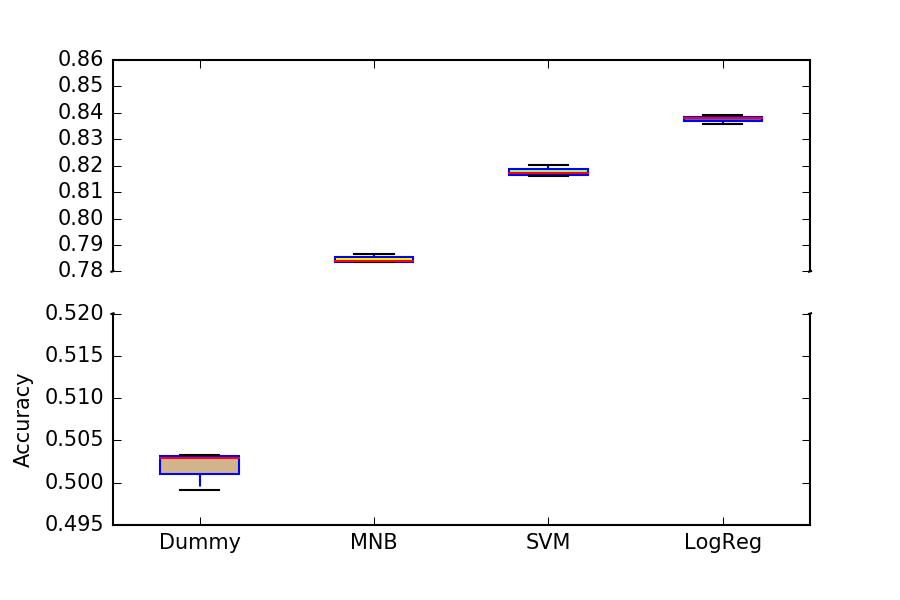
\includegraphics[width=\columnwidth]{plots/Classifiers_boxplots2.png}
    \caption{Accuracies for each investigated classifiers (default hyperparameters from \textit{scikit-learn} modules) including its optimal pre-processing.}
    \label{fig:classifiers}
\end{figure}
% \vspace{0.3cm}
It is thus clear that replacing multiple occurrences of two words improves the classification accuracy of LogReg and SVM. Another determining hyperparamter is the \textit{n-grams} while feature generation. 
%\ref{fig:all_models_boxplots} 
\subsection{Hyperparameter optimization}
The \textit{CountVectorizer()} and \textit{TfidfTransfromer()} from \textit{scikit-learn} have multiple hyperparameters that can be tuned. 
A first hyperparameter is \texttt{N-gram}, already described in the Methodology section. 
Other hyperparameters are \texttt{max\textunderscore df}, a threshold to cut off highly frequent words; and \texttt{min\textunderscore df}, a threshold to clip off very rare words. 
Moreover, the maximal amount of features, \texttt{max\textunderscore features}, can be set. 
Another hyperparameter is the inverse L2 regularization strength (\texttt{C}) of the LogReg. \\
In order to search through the complete landscape of each hyperparameter, we first apply a random search using  \textit{scikit-learn}'s \textit{RandomSearchCV()}, on a wide range of hyperparameters to get an initial idea of the optimal parameters for the full dataset. 
The returned values are reported in Table \ref{tab:coarse_hyper} and give an accuracy of $0.8686 \pm 0.0023$ on the full dataset.
% \begin{table}[H]
% \centering
% \resizebox{.5\columnwidth}{!}{
% % \tiny
% \begin{tabular}{{l}c} 
% \hline
% \rule{0pt}{2mm}
% \textbf{hyperparameter} & \textbf{value}\\
% \hline
% \texttt{max\_features}			&$None$ \\
% \texttt{ngram\_range}			&$(1,3)$ \\
% \texttt{max\_df}				&$\approx 0.9261$ \\
% \texttt{min\_df}				&$4$ \\
% \texttt{C}						&$\approx 2.1544$ \\
% \hline
% \end{tabular}
% }
% \caption{\label{tab:coarse_hyper}Hyperparameters returned by coarse RandomSearchCV().}
% \end{table}

% \vspace{0.3cm}
\begin{table}[!htb]

    \begin{subtable}{.48\linewidth}
      \caption{\label{tab:coarse_hyper}}
      \centering
       \begin{tabular}{{l}c} 
\hline
\rule{0pt}{2mm}
\textbf{hyperparameter} & \textbf{value}\\
\hline
\texttt{max\_features}			&$None$ \\
\texttt{ngram\_range}			&$(1,3)$ \\
\texttt{max\_df}				&$\approx 0.9261$ \\
\texttt{min\_df}				&$4$ \\
\texttt{C}						&$\approx 2.1544$ \\
\hline
\end{tabular}
    \end{subtable}%
    \begin{subtable}{.48\linewidth}
      \centering
       \caption{\label{tab:fine_hyper}}
        \begin{tabular}{{l}c}
\hline
\rule{0pt}{2mm}
\textbf{hyperparameter} & \textbf{value}\\
\hline
\texttt{max\_features}			&$None$ \\
\texttt{ngram\_range}			&$(1,3)$ \\
\texttt{max\_df}				&$\approx 0.9261$ \\
\texttt{min\_df}				&$4$ \\
\texttt{C}						&$3.41$ \\
\hline
\end{tabular}
    \end{subtable} 
        \caption{Hyperparameters returned by (a) coarse RandomSearchCV() and (b) fine sampling around the optimal range.}

\end{table}
% \vspace{0.3cm}
We then perform a fine-grain search on the small dataset to optimize the hyperparameter \texttt{C} for Logistic Regression. 
Fig. \ref{fig:C_Landscape} illustrates the testing accuracy peak of $0.8534 \pm 0.0039$ at around $\texttt{C} = 3.41$ on the small dataset that yield an accuracy of $ 0.8739 \pm 0.0017$ on the full dataset after 3-fold CV.
The final hyperparameters are then the ones specified in Table \ref{tab:fine_hyper} with \texttt{1783165} features.

%\textbf{We still have to write about the ROC curve!}
To analyze the classification performance of our classification system, we plot the \textit{receiver operating characteristic (ROC) curve} \ref{fig:ROC}. 
This is the true positive rate against the false positive rate for the different possible cut-points. 
Generally, the closer the curve to the left upper corner of the ROC space, the more accurate the classification; and the closer the curve to the diagonal, the less accurate the classification. 
Therefore, the \textit{area under the curve (AUC)} is a measure of classification accuracy.
One can see that the AUC of the mean ROC over three folds is $0.92 \pm 0.0047$, showing that our classification holds an accuracy of $92\%$.
%TF-IDF: ngram, maxdf, mindf, max features
%Logistic regression holds multiple hyperparameters one needs to tune. C
% \vspace{0.3cm}
\begin{figure}[tbp]
  \centering
  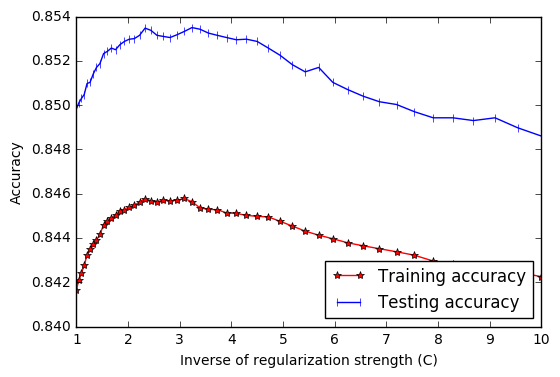
\includegraphics[width=\columnwidth]{plots/C_value_vs_accuracy.png}
  \caption{Landscape of the hyperparameter \texttt{C} of Logistic Regression classifier on features obtained from optimized TF-IDF.}
  \vspace{-3mm}
  \label{fig:C_Landscape}
\end{figure}
% \vspace{0.3cm}
% \vspace{0.3cm}
\begin{figure}[tbp]
  \centering
  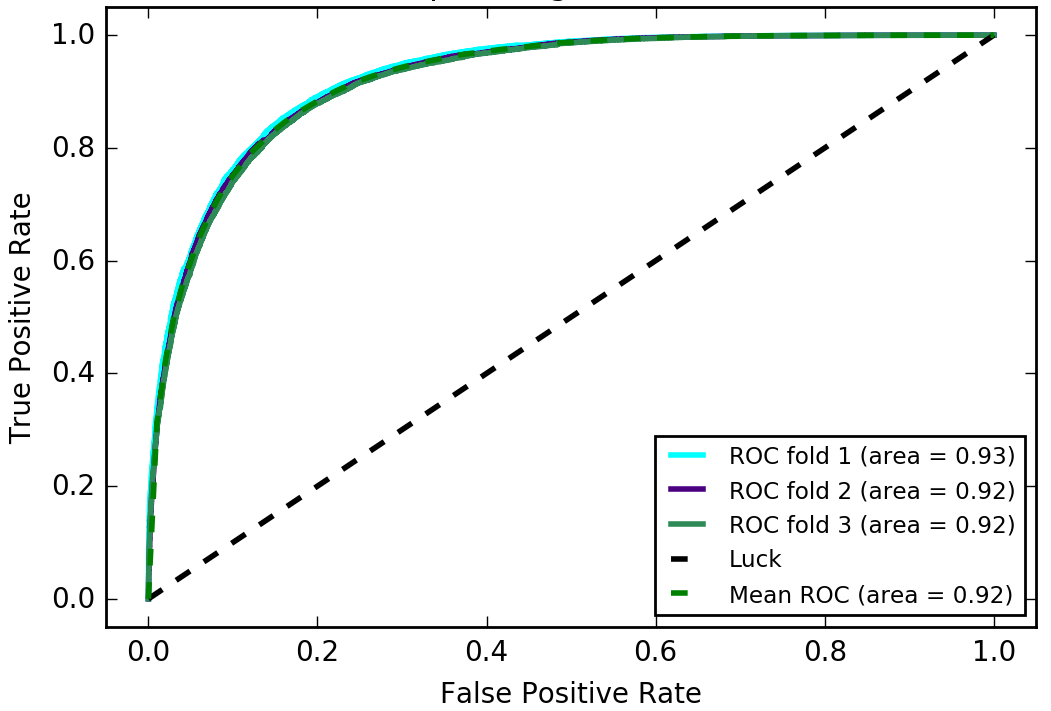
\includegraphics[width=\columnwidth]{plots/ROC_logreg.png}
  \caption{ROC curve ilustrating the LogReg classifier performances over 3-CV fold.}
  \vspace{-3mm}
  \label{fig:ROC}
\end{figure}
% ----------
\iffalse
\subsection{Figures and Tables}
% \vspace{0.3cm}


\texttt{variance curve to explain why downloading more datapoints was a good or bad choice?}\\

\texttt{accuracy vs different preprocessing step plot (for tfidf, may be?) (may differ for different classifiers as naive preferred removal of stop words, others did not)}\\

\texttt{accuracy vs classifier plot (for all the models)}\\

\texttt{accuracy vs model with their corresponding best classifier plot}\\

\texttt{hyperparameter optimization using random search}
\fi

% \vspace{0.3cm}
\section{Discussion}
%TODO - what is good, what is bad, challenges we faced, what could be improved
Starting with different types of embeddings, the TF-IDF embedding gives the best baseline results. 
This is surprising as the popular GloVe algorithm can be regarded as a state-of-the-art. 
Thus, we speculate that GLoVe would have given comparable accuracies as TF-IDF with proper data pre-processing and/or using computationally expensive Neural Networks.\\ %\textbf{The fastText script gives good accuracies, but optimization was difficult given the limited information we had about hyper parameters}.\\
Despite the fact that the current state-of-the-art\cite{deriu2016swisscheese} makes use of Convolutional Neural Networks, the lack of computational power to train them is not negligible.
This is why we chose the TF-IDF: it is ease to be implemented and requires very small computational power. 
The strength of our final model is its computational simplicity compared to large Neural Networks. 
Our model can be trained in a moderate time interval (50 minutes on a laptop powered by 2.2-GHz Intel Core i7 processor and 16 GB of RAM) while still producing impressive predictions. 
This is achieved by optimizing the model on different levels from the data pre-processing up to the classifier. 
We have reported only the pre-processing steps that actually increase the accuracy alone, ensuring a better prediction. 
The features were engineered using several tricks such as N-grams for better capturing the meaning of a tweet. 
All hyperparamters have been tweaked extensively using a first round a coarse-grained global "random" search, and in a second round a very fine tuning on a small set of possible parameters around the best result from the first round. Finally, we have \textit{1,783,165} features that lead to a highly optimized Twitter sentiment analyzer with an accuracy of $0.8739 \pm 0.0017$ on 3-fold CV on the full dataset using Logistic Regression. Here each feature represent a token in the vocabulary with one or more words.\\
Naturally, there exits further possibility to improve our sentiment analyzer.
Considering the free available modules from the Natural Language Toolkit (NLTK)\cite{Loper:2002:NNL:1118108.1118117} for text pre-processing and classification, one can think of introducing extra levels of information such as the Part-Of-Speech tagging or Named-entity recognition.\\
Moreover, it would be interesting to see the pre-processing steps applied to tweets that are then fed into a powerful method, such as CNNs.
% \vspace{0.3cm}

\section{Conclusion}
In this report, we described and compared several sentiment classifiers optimized towards predicting the sentiment polarity of tweets. 
Our approach is based on simple classification scheme in contrast to highly complex Neural Networks and therefore computationally quite cheap.
Though it relies on a large amount of training data.
After pre-processing, feature engineering and classifier optimization we were able to build a sentiment analyzer trained in a moderate time window while holding a good performance in terms of accuracy.
% \vspace{0.3cm}
% \section*{Acknowledgements}
% The author thanks Christian Sigg for his careful reading and helpful
% suggestions.
% \vspace{0.3cm}
\bibliographystyle{IEEEtran}
\bibliography{BIB.bib}
% \vspace{0.3cm}
\end{document}